
\section{Deep finite neuron functions, adaptivity and spectral
  accuracy}  
\label{sec:deep-fnm} 
In this section, we will study deep finite neural functions through
the framework of  deep neural networks and then discuss its adaptive
and spectral accuracy properties. 

\subsection{Deep finite neuron functions}
Given $d, \ell\in\mathbb{N}^+$, 
$
n_1,\dots,n_{\ell}\in\mathbb{N} \mbox{ with }n_0=d, n_{\ell+1}=1, 
$
\begin{equation}\label{thetamap}
\theta^i(x)=\omega_i\cdot x + b_i,\quad \omega_i\in \mathbb{R}^{n_{i+1}\times n_i},\ b\in \mathbb{R}^{n_{i+1}},
\end{equation}
and the activation function ${\rm ReLU}^k$, define
a  deep finite neuron function $u(x)$ from $\mathbb{R}^d$ to $\mathbb{R}$  as follows:
\begin{align*}
f^0(x)   &=\theta^0(x) \\ 
f^{i}(x) &= [  \theta^{i} \circ \sigma ](f^{i-1}(x)) \quad i = 1:\ell \\
f(x) &= f^\ell(x). \\
\end{align*}
The following more concise notation is often used in computer science literature:
\begin{equation}
\label{compress-dnn}
f(x) = \theta^{\ell}\circ \sigma \circ \theta^{\ell-1} \circ \sigma \cdots \circ \theta^1 \circ \sigma \circ \theta^0(x),
\end{equation}
here $\theta^i: \mathbb{R}^{n_{i}}\to\mathbb{R}^{n_{i+1}}$ are linear
functions as defined in \eqref{thetamap}.  Such a deep neutral network
has $(\ell+1)$-layer DNN, namely $\ell$-hidden layers. The size of
this deep neutral network is $n_1+\cdots+n_{\ell}$.

Based on these notation and connections, define deep finite neuron
functions with activation function $\sigma={\rm ReLU}^k$ by
\begin{equation}
\label{NNL}
\Sigma^k_{n_1,n_2,\ldots, n_\ell}=\bigg\{ f^{\ell}(x) = \theta^\ell (x^{\ell}), 
 \mbox{ with } W^i\in \mathbb R^{n_{i+1}\times
	n_{i}}, b^i\in\mathbb R^{n_i}, i=0:\ell, n_0=d, n_{\ell+1}=1\bigg\}  
\end{equation}
Generally, we can define the $\ell$-hidden layer neural network as:
\begin{equation}
\Sigma^k_{\ell,n}:= \bigcup_{n_1, n_2, \cdots, n_{\ell}\ge 1}\Sigma^k_{n_1,n_2,\ldots, n_\ell}.
\end{equation}
For $\ell=2$, functions in $\Sigma^k_{1,n}$ consist of piecewise polynomials of degree $k^2$ on a finite neuron grids whose boundaries are level sets of quadratic polynomials, see Fig \ref{fig:3}.
\begin{figure}[!ht]
\begin{center} 
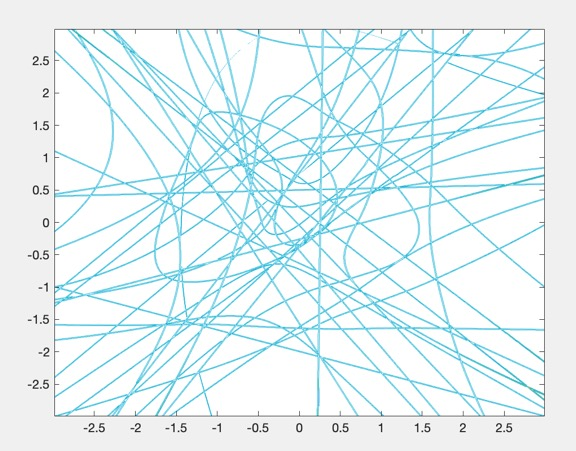
\includegraphics[width=.3\textwidth]{6DL/figures/2t20t20-1.jpg}   
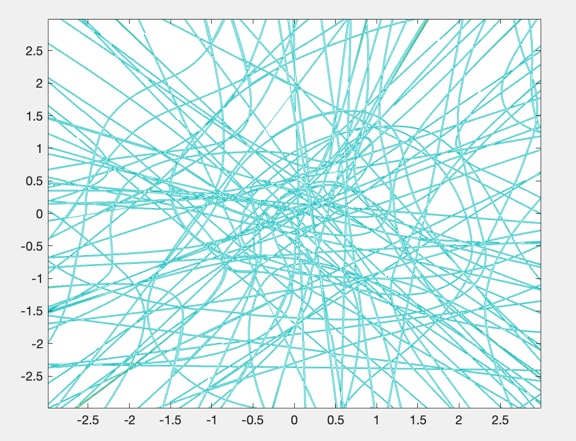
\includegraphics[width=.3\textwidth]{6DL/figures/2t40t40-1.jpg}
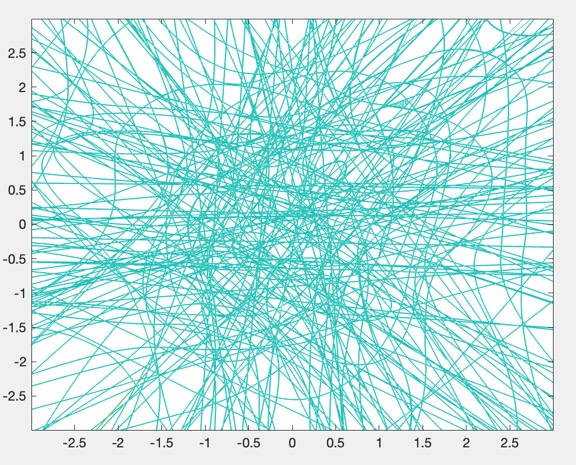
\includegraphics[width=.28\textwidth]{6DL/figures/2t60t60-1.jpg}    
\caption{Hidden finite neuron grids with $\ell=2$}
\label{fig:3}
\end{center}
\end{figure} 

\subsection{Reproduction of polynomials and spectral accuracy}
One interesting property of the ReLU$^k$-DNN is that it reproduces
polynomials of degree $k$.  
\begin{lemma}
Given $k\ge 2$, $q\ge 2$, there exist $\ell\ge 1$, $n_1, \cdots, n_\ell$ such that
$$
\mathbb{P}_q\subset \Sigma^k_{\ell,n},
$$
where $\mathbb{P}_q$ is the set of all polynomials with degree not larger than $q$.
\end{lemma}
\begin{proof}
	Here we provide a sketch of the proof. We first notice that
	$$
	x^k = {\rm ReLU}^k(x) + (-1)^k{\rm ReLU}^k(-x) \in \Sigma^k_{2}, \quad \forall x \in \mathbb{R},
	$$
	for any $k\ge2$. In addition, there exists $a_i, b_i, c_i \in \mathbb{R}$ such that
	$$
	x^2 = \sum_{i=1}^{k+1} c_i(a_i x + b_i)^k  \in \Sigma^k_{2(k+1)}, \forall x \in \mathbb{R}.
	$$
	Thus, we have
	$$
	x\times y = \frac{(x+y)^2 - (x-y)^2}{4} \in \Sigma^k_{2, 4(k+1)}, \forall x,y \in \mathbb{R}.
	$$
	This shows that
	\begin{equation}\label{key}
	\begin{split}
	x_1^{\alpha_1}x_2^{\alpha_2}\cdots x_d^{\alpha_d} 
	&= x_1 \times x_1^{\alpha_1-1}x_2^{\alpha_2}\cdots x_d^{\alpha_d} \\
	&\vdots \\
	&= x_1\times \left(x_1 \times \left(x_1 \cdots \times \left(x_d\times (x_d \times x_d)\right)\cdots\right)\right).
	\end{split}
	\end{equation}
	Thereby, any monomial $x_1^{\alpha_1}x_2^{\alpha_2}\cdots x_d^{\alpha_d}$ with degree $|\alpha| = \sum_{i=1}^d \alpha_i$ can be represented by a deep ${\rm ReLU}^k$ neural network.
\end{proof}
For a more detailed proof of the above result, we refer to \cite{li2019better}. 

\begin{theorem}\label{thm:spectral}
Let  ${\rm ReLU}^k$ be the activation function, and $\dnn_\ell^k(N)$ be the DNN model with $\ell$ hidden layers. 
There exists some $\ell$ such that
\begin{equation}\label{eq:spectral}
\inf_{v_n\in \Sigma^k_{\ell,n}}\|u-v_n \|_{H^m(\Omega)} \lesssim
\inf_{v_n\in \mathbb{P}_{k^\ell}} \|u-v_n\|_{H^m(\Omega)},
\end{equation} 
\end{theorem}
Estimate \eqref{eq:spectral} indicates that the deep finite neuron function may provide spectral approximate accuracy.

\subsection{Reproduction of linear finite element functions and adaptivity}
The deep neural network with ReLU activation function have
been much studied in the literature and most widely used in practice.
One interesting fact is that ReLU-DNN is simply piecewise linear
functions.  More specifically, recall the results in Section \ref{sec:reluFEM}.

\begin{lemma}
Assume that ${\cal T}_h$ is a simplicial finite element grid of $N$ elements, in which any 
union of simplexes that share a same vertex is convex, any linear finite element function on this grid 
can be written as a ReLU-DNN with at most $\mathcal
  O(d)$ hidden layers. The number of neurons is at most
  $\mathcal{O}(\kappa^dN)$ for some constant $\kappa\ge 2$ depending
  on the shape-regularity of $\mathcal T_h$.  The number of non-zero
  parameters is at most $\mathcal{O} (d\kappa^dN)$.
\end{lemma}

The above result indicate that the deep finite neuron functions can
reproduce any linear finite element functions.  Given the adaptive
feature and capability of finite element methods, we see that the
finite neuron method can be at least as adaptive as finite element method.

\section{Elliptic boundary value problems of order $2m$}\label{sec:model}
Let $\Omega\subset \mathbb{R}^d$ be a bounded domain with a
sufficiently smooth boundary $\partial\Omega$.  For any integer $m\ge
1$, we consider the following model $2m$-th order partial differential
equation with certain boundary conditions:
%\begin{equation}\label{equ:2mpde}(-\Delta)^m u +u = f \qquad \mbox{in }\Omega.\end{equation}
\begin{equation} \label{2mPDE}
\left\{
  \begin{array}{rccl}\displaystyle
Lu &=& f &\mbox{in }\Omega, \\
B^k(u) &= &0 & \mbox{on }\partial\Omega \quad(0\le k\le m-1),
  \end{array}
\right.
\end{equation}
where $L$ is a partial differential operator as follows
\begin{equation}\label{Lu}
Lu= \sum_{|\alpha|=m}(-1)^m\partial^\alpha (a_\alpha(x)\,\partial^\alpha\,u) +a_0(x)u,
 \end{equation} 
and ${\boldsymbol{\alpha}}$ denotes $n$-dimensional multi-index ${\boldsymbol{\alpha}}
= (\alpha_1, \cdots, \alpha_n)$ with
$$
|{\boldsymbol{\alpha}}| = \sum_{i=1}^n \alpha_i, \quad
\partial^{\boldsymbol{\alpha}} = \frac{\partial^{|{\boldsymbol{\alpha}}|}}{\partial x_1^{\alpha_1}
\cdots \partial x_n^{\alpha_n}}.
$$
For simplicity, we assume that $a_\alpha$ are strictly positive and smooth functions on
$\Omega$ for  $|\alpha|=m$ and $\alpha=0$, namely, $\exists \alpha_0>0$, such that 
\begin{equation}\label{ass:1}
a_\alpha(x), a_0(x)\ge \alpha_0,\,\, \forall x\in\Omega,\,\,|\alpha|=m.
 \end{equation} 
Given a nonnegative integer
$k$ and a bounded domain $\Omega\subset \mathbb{R}^d$, let 
$$
H^k(\Omega):=\left\{v\in L^2(\Omega), \partial^\alpha v\in L^2(\Omega), |\alpha|\le k\right\}
$$
be standard Sobolev spaces with norm and seminorm given respectively by 
$$
 \|v\|_k:=\left(\sum_{|\alpha|\le k} \|\partial^\alpha v\|_0^2\right)^{1/2}, \quad  |v|_k:=\left(\sum_{|\alpha|= k} \|\partial^\alpha v\|_0^2\right)^{1/2}.
$$
For $k=0$, $H^0(\Omega)$ is the standard $L^2(\Omega)$ space
with the inner product denoted by $(\cdot, \cdot)$.  Similarly, for
any subset $K\subset \Omega$, $L^2(K)$ inner product is denoted by
$(\cdot, \cdot)_{0,K}$.  We note that, by well-known property of Sobolev space,  the assumption \eqref{ass:1} implies that
\begin{equation}
  \label{avv}
a(v,v)\gtrsim \|v\|^2_{m,\Omega}, \forall v\in H^m(\Omega).
\end{equation}

The boundary value problem \eqref{2mPDE} can be cast into an
equivalent optimization or a variational problem as described below for some approximate subspace $V\subset H^m(\Omega)$.
\begin{description}
\item[Minimization Problem M:] Find $u\in V$ such that 
\begin{equation}
\label{minJv}
J(u)=\min_{v\in V} J(v),
\end{equation}
\noindent or
\item[Variational Problem V:]  Find  $u\in V$ such that 
\begin{equation}\label{m-vari} 
a(u,v) = \langle f, v\rangle \quad \forall v \in V.
\end{equation}
\end{description}
The bilinear form $a(\cdot,\cdot)$ in \eqref{m-vari}, the objective
functional $J(\cdot)$ in \eqref{minJv} and the functional space $V$
depend on the type of boundary condition in \eqref{2mPDE}. 

One popular type of boundary conditions are Dirichlet boundary
condition when $B^k=B_D^k$ are given by the following Dirichlet type
trace operators
\begin{equation}\label{BD}
B_D^k(u):=\left.\frac{\partial^k u}{\partial
    \nu^k}\right|_{\partial\Omega}\quad (0\le k\le m-1),
\end{equation}
with $\nu$ being the outward unit normal vector of $\partial\Omega$. The Dirichlet boundary
value problem as follows:
\begin{equation} \label{m-BD}
\left\{
  \begin{array}{rccl}\displaystyle
Lu &=& f &\mbox{in }\Omega, \\
B_{D}^k(u) &= &0 & \mbox{on }\partial\Omega \quad(0\le k\le m-1).
  \end{array}
\right.
\end{equation}


For the aforementioned Dirichlet boundary condition, the elliptic
boundary value problem \eqref{2mPDE} is equivalent to \eqref{minJv} or
\eqref{m-vari} with $V=H^m_0(\Omega)$ and 
\begin{equation}
  \label{auv}
a(u,v) := \sum_{|\alpha | = m}(a_\alpha\partial^{\alpha}u, \partial^{\alpha}v)_{0,\Omega} +(a_0u,v)\quad \forall
u, v \in V,
\end{equation}
and 
\begin{equation}
  \label{Jv}
J(v)=\frac12 a(v,v) -\int_{\Omega} fv dx.  
\end{equation}

We next discuss about the pure Neumann boundary conditions 
for general PDE operator \eqref{Lu} when $m\ge 2$.  We first begin our discussion
with the following simple result. 
\begin{lemma} \label{lem:BDBNdual}
For each $k=0,1,\ldots,m-1$, there exists a bounded linear differential operator of order $2m-k-1$:
\begin{equation}
    \label{BN}
B_N^k: H^{2m}(\Omega)\mapsto L^2(\partial\Omega)    
  \end{equation}
such that the following identity holds
$$
(Lu,v)=a(u,v)-\sum_{k=0}^{m-1}\langle B_N^k(u),B_D^k(v)\rangle _{0,\partial\Omega}.
$$
Namely
\begin{equation}
\label{BDBNdual}
\sum_{|\alpha|=m}(-1)^m\left(\partial^\alpha
  (a_\alpha\,\partial^\alpha\,u),\,v\right) _{0,\Omega}
=\sum_{|{\boldsymbol{\alpha}}|=m}\left(a_\alpha\partial^{\boldsymbol{\alpha}}\,u, \partial^{\boldsymbol{\alpha}} v\right) _{0,\Omega}
-\sum_{k=0}^{m-1}\langle B_N^k(u),B_D^k(v)\rangle _{0,\partial\Omega}
\end{equation}
for all $u\in H^{2m}(\Omega), v\in  H^{m}(\Omega)$. Furthermore, 
\begin{equation}\label{equ:regassum}
\sum_{k=0}^{m-1}\|B_D^k(u)\|_{L^2(\partial\Omega)}+\sum_{k=0}^{m-1}\|B_N^k(u)\|_{L^2(\partial\Omega)}\lesssim \|u\|_{2m, \Omega}.
\end{equation}
\end{lemma}
Lemma \ref{lem:BDBNdual} can be proved by induction with
respect to $m$.  We refer to \cite{lions2012non} (Chapter 2) and \cite{chen2020nonconforming} for a proof on a similar identity.

In general the explicit expression of $B_N^k$ can be quite
complicated.  Let us get some idea by looking at some simple examples
with the following special operator:
\begin{equation}
  \label{Delta-m}
Lu=(-\Delta)^m u+u,
\end{equation}
and 
\begin{equation}
a(u,v)= \sum_{|\alpha | = m}(a_\alpha\partial^{\alpha}u, \partial^{\alpha}v)_{0,\Omega} +(a_0u,v)\quad \forall
u, v \in V.
\end{equation}

\begin{itemize}
\item For $m=1$, it is easy to see that $B_N^0 u=\frac{\partial u}{\partial
    \nu}|_{\partial\Omega}$.
\item For $m=2$ and $d=2$, see \cite{chien1980variational}: 
$$
B_N^0 u= \frac{\partial}{\partial \nu}\left(\Delta
  u+\frac{\partial^2u}{\partial
    \tau^2}\right)-\frac{\partial}{\partial
  \tau}\left({\kappa_\tau}\frac{\partial u}{\partial \tau}\right)|_{\partial\Omega}~~\hbox{and}~~B_N^1 u=\frac{\partial^2u}{\partial \nu^2}|_{\partial\Omega},
$$
   with $\tau$ being the
anti-clockwise unit tangential vector, and $\kappa_\tau$ the curvature
of $\partial\Omega$. 
\end{itemize} 

We are now in a position to state that the pure Neumann boundary value
problems for PDE operator \eqref{Lu} as follows.
\begin{equation} \label{m-BN}
\left\{
  \begin{array}{rccl}
Lu &=& f &\mbox{in }\Omega, \\
B_{N}^k(u) &= &0 & \mbox{on }\partial\Omega \quad(0\le k\le m-1).
  \end{array}
\right.
\end{equation}
Combining the trace theorem for $H^m(\Omega)$, see \cite{adams2003sobolev}, and Lemma
\eqref{lem:BDBNdual},  it is easy to see that 
\eqref{minJv} is equivalent to 
\eqref{m-BN} 
with $V=H^m(\Omega)$. 

For a given parameter $\delta>0$, we next consider the following
problem with mixed boundary condition: 
\begin{equation} \label{equ:delta}
\left\{
\begin{aligned}
Lu_{\delta} &= f \qquad \mbox{in }\Omega, \\
B_D^k(u_{\delta})+\delta B_N^k(u_\delta)  &= 0, \ \ 0\le k\le m-1.
\end{aligned}
\right.
\end{equation}
It is easy to see that \eqref{equ:delta} is equivalent to the following problem: Find $u_\delta\in H^m(\Omega)$, such that 
\begin{equation}\label{equ:varpdelta}
J_{\delta}(u_{\delta})=\min_{v\in H^m(\Omega)} J_{\delta}(v).
\end{equation}
where
\begin{equation}\label{J-delta}
J_\delta(v)={1\over 2}a_\delta(v,v)-(f,v)
\end{equation}
and
\begin{equation}\label{a-delta}
a_\delta(u,v)=a(u,v)+\delta^{-1}\sum_{k=0}^{m-1}\langle B_D^k(u), B_D^k(v)\rangle_{0,\partial\Omega}.
\end{equation}
In summary, we have 
\begin{lemma}
The following equivalences hold:
\begin{enumerate}
\item $u$ solves for \eqref{m-BD} or \eqref{m-BN} if and only if $u$ solves
\begin{equation}\label{m-mini}
J(u)=\min_{v\in V} J(v)
\end{equation}
 with $V=H^m_0(\Omega)$ or  $V=H^m(\Omega)$,
\item $u_\delta$ solves for \eqref{equ:delta}  if and only if $u_\delta$ solves 
$$
\displaystyle J_\delta(u_\delta)=\min_{v\in V} J_\delta(v)
$$ 
with $V=H^m(\Omega)$. 
\end{enumerate}
\end{lemma}


\begin{lemma} \label{lem:JvJu}
Assume that $u\in V$ be solution of \eqref{m-BD} or \eqref{m-BN} and $u_\delta\in V$ be the solution of \eqref{equ:varpdelta}, then
the following identities hold:
\begin{equation}\label{vuidentity1}
\|v-u\|_{a}^2=J(v)-J(u)\quad \forall v\in V,
\end{equation}
and
\begin{equation}\label{vuidentity2}
\|v-u_\delta\|_{a,\delta}^2=J_{\delta}(v)-J_{\delta}(u_{\delta})\quad \forall v\in V. 
\end{equation}
Here
\begin{equation}
  \label{a-norm}
\|v\|_{a}^2=a(v,v),\quad \|v\|_{a,\delta}^2=a_\delta(v,v).
\end{equation}
\end{lemma}
\begin{proof}
Let $u$ be the solution of \eqref{minJv}. Given $v\in V$, consider the quadratic function of $t$:
$$
g(t)=J(u+t(v-u)).
$$
It is easy to see that 
$$
0=\arg\min_{t}g(t), \quad g'(0)=0,
$$
and
$$
J(v)-J(u)=g(1)-g(0)=g'(0)+{1\over2}g''(0)=\|v-u\|_{a}^2.
$$
This completes the proof of \eqref{vuidentity1}. The proof of \eqref{vuidentity2} is similar. 
\end{proof} 

\begin{lemma}\label{Nitchtrick}
  Let $u$ be the solution of \eqref{m-BD} and $u_\delta$ be the solution of \eqref{equ:delta}. Then 
  \begin{align}\label{diff:uudelta}
\|u-u_\delta\|_{a,\delta} \lesssim\sqrt{\delta}  \|u\|_{2m,\Omega}.
\end{align}
\end{lemma}
\begin{proof}
Let $w=u-u_{\delta}$ and we have 

\begin{equation} \label{equ:diff}
\left\{
\begin{aligned}
Lw &= 0 \qquad \mbox{in }\Omega, \\
B_D^k(w)+\delta B_N^k(w)  &= \delta B_N^k(u),\ \ 0\le k\le m-1.
\end{aligned}
\right.
\end{equation}
By Lemma \ref{lem:BDBNdual}, and \eqref{equ:diff},  we have 
\begin{align}
0&=(Lw, w)
\\
&=\sum_{|\alpha|=m}(a_\alpha\partial^\alpha w, \partial^\alpha w)-\sum_{k=0}^{m-1}\int_{\partial \Omega}B_N^k(w)B_D^k(w) ds+(a_0w, w)
\\
&=\sum_{|\alpha|=m}(a_\alpha\partial^\alpha w, \partial^\alpha w)+ \sum_{k=0}^{m-1} \int_{\partial \Omega}(\delta^{-1}B_D^k(w)-  B_N^k(u) )B_D^k(w) ds+(a_0w, w),
\end{align}
implying
\begin{align}
&a(w, w)+ \delta^{-1}\sum_{k=0}^{m-1}\int_{\partial \Omega}B_D^k(w)^2 ds
=
\sum_{k=0}^{m-1}\int_{\partial \Omega}B_N^k(u)B_D^k(w) ds.
\end{align}
By Cauchy inequality, we have 
\begin{align}
a(w,w)+\delta^{-1}\sum_{k=0}^{m-1}\|B_D^k(w)\|^2_{L^2(\partial \Omega)}
\le& \sum_{k=0}^{m-1}\|B_N^k(u) \|_{L^2(\partial \Omega)}\|B_D^k(w)\|_{L^2(\partial \Omega)}
\\
\le& 2\delta  \sum_{k=0}^{m-1}\|B_N^k(u) \|^2_{L^2(\partial \Omega)}+\frac12 \delta^{-1} \sum_{k=0}^{m-1} \|B_D^k(w)\|^2_{L^2(\partial \Omega)},
\end{align}
which implies
\begin{align}
a(w,w)+\frac12 \delta^{-1}\sum_{k=0}^{m-1}\|B_D^k(w)\|^2_{L^2(\partial \Omega)}\le 2\delta  \sum_{k=0}^{m-1}\|B_N^k(u) \|^2_{L^2(\partial \Omega)}.
\end{align}
By the definition of $\|\cdot\|_{a,\delta}$ and noting that $w=u-u_\delta$, we have 
\begin{align}\label{diff:uudelta1}
\|u-u_\delta\|_{a,\delta}^2\le 4\delta  \sum_{k=0}^{m-1}\|B_N^k(u) \|^2_{L^2(\partial \Omega)}.
\end{align}
Combing this with \eqref{equ:regassum}, then completes the proof.
\end{proof}

\begin{lemma}\label{Regularity}
For any $s\ge -m$ and  $f\in H^s(\Omega)$, the solution $u$
  of \eqref{m-BD} or \eqref{m-BN} satisfies $u\in H^{2m+s}(\Omega)$ and 
  \begin{equation}
    \label{regularity}
\|u\|_{2m+s,\Omega}\lesssim     \|f\|_{s,\Omega}.
  \end{equation}
\end{lemma}
We refer to \cite{lions2012non} (Chapter 2, Theorem 5.1 therein) for a detailed proof. 

Following from \eqref{regularity} and \eqref{embend}, we have 
\begin{lemma} For any $s\ge -m$,  $\epsilon >0$, 
 and  $f\in H^s(\Omega)$, the solution $u$
  of \eqref{m-BD} or \eqref{m-BN} satisfies
  \begin{equation}
  \label{Barron-regularity}
\|u\|_{B^{m+1}(\Omega)}\le   \|f\|_{-m+\frac{d}{2}+1+\epsilon,\Omega}.
\end{equation}
\end{lemma}


\section{The finite neuron method and error estimates}\label{sec:FNM}
Let $V_n\subset V$ be a subset of $V$ defined by \eqref{VkN} which may not be a linear
subspace. Consider the the discrete problem of \eqref{m-mini}:
\begin{equation}
  \label{m-mini-VN}
\mbox{Find $u_n\in V_n$ such that } J(u_n)=\min_{v_n\in V_n}J(v_n).
\end{equation}
It is easy to see that the solution to \eqref{m-mini-VN} always exists (for deep
neural network functions as defined below), but may not be unique.

\begin{theorem}\label{thm:best} Let $u\in V$ and $u_n\in V_n$ be solutions to
  \eqref{m-BN} and \eqref{m-mini-VN} respectively.   Then
  \begin{equation}
    \label{best-approx}
\|u-u_n\|_a=\inf_{v_n\in V_n}\|u-v_n\|_a.
  \end{equation}
\end{theorem}
\begin{proof}
By  Lemma~\ref{lem:JvJu}, we have
$$
\|u_n-u\|_a^2=J(u_n)-J(u)\le J(v_n)-J(u)=\|v_n-u\|_a^2,\quad\forall v\in V_n.
$$
The proof is completed.
\end{proof}
We obtain the following result.
\begin{theorem}
Let $u\in V$ and $u_n\in V_n$ be solutions to
\eqref{m-BN} and \eqref{m-mini-VN} respectively.  Then for arbitrary $\epsilon>0$, we have
\begin{equation}\label{error:N}
\|u-u_n\|_a \lesssim 
(\|f\|_{L^2(\Omega)}+\|f\|_{\mathcal{K}_1(\mathbb{D})})
\begin{cases}
n^{-{1\over 2}-{2(k-m)+1\over 2d}}&m< k,
\\
n^{m-k-1}& m\ge k.
\end{cases} 
\end{equation}
\end{theorem}
By \eqref{best-approx},  and the embedding of spectral Barron space  into Sobolev space, namely Lemma \ref{smoothness-lemma}, the regularity result \eqref{regularity}, we get the proof. 

Next we consider the discrete problem of \eqref{equ:varpdelta}:
\begin{equation}
\label{min:uN}
\mbox{Find $u_n\in V_n$ such that } J_\delta(u_n)=\min_{v_n\in V_n}J_\delta(v_n).
\end{equation}

\begin{lemma}
For any given number $\delta$, let $u_\delta$ be the solution of \eqref{equ:delta} and
  $u_n$ be the solution of \eqref{min:uN}, respectively. We have
  \begin{equation}
  \label{eq:1}
\|u_n-u_\delta\|_{a,\delta} \lesssim (1+ \delta^{-\frac12})  \inf_{v_n\in
  V_n} \|v_n-u_\delta\|_{m,\Omega}. 
  \end{equation}
\end{lemma}
\begin{proof}
First of all, by Lemma~\ref{lem:JvJu} and the variational property, it holds that
\begin{align}\label{eq:min}
\|u_n-u_\delta\|_{a,\delta}^2=J_{\delta}(u_n)-J_{\delta}(u_{\delta})\le J_{\delta}(v_n)-J_{\delta}(u_{\delta})
=\|v_n-u_\delta\|_{a,\delta}^2, \quad \forall\,v_n\in V_n.
\end{align}
Further, for any $v_n\in V_n$, by the definition of $\|\cdot\|_{a,\delta}$ and trace inequality, we have 
$$
\|v_n-u_\delta\|_{a,\delta}\lesssim  \|v_n-u_\delta\|_{m,\Omega}+\delta^{-\frac12} \|v_n-u_\delta\|_{0,\partial\Omega}\lesssim (1+\delta^{-\frac12})\|v_n-u_\delta\|_{m,\Omega}.
$$
This completes the proof. 
\end{proof}

\begin{theorem}\label{thm:bestD}
  Let $u$ be the solution of \eqref{m-BD} and
  $u_n$ be the solution of \eqref{min:uN}, respectively. We have
  \begin{equation}
  \label{eq:13}
\|u-u_n\|_{a,\delta} \lesssim (1+ \delta^{-\frac12})  \inf_{v_n\in
  V_n} \|v_n-u\|_{m,\Omega}
+\sqrt{\delta}  \|f\|_{L^2(\Omega)}. 
  \end{equation}
\end{theorem}
\begin{proof}
First, by triangle inequality and \eqref{eq:min}, for any $v_n\in V_n$, we have
\begin{align}
\|u_n-u\|_{a,\delta}&\le  \|u_n-u_\delta\|_{a,\delta}+\|u_\delta-u\|_{a,\delta}\\
&\le \|v_n-u_\delta\|_{a,\delta}+\|u_\delta-u\|_{a,\delta}\\
&\le  \|v_n-u\|_{a,\delta}+2\|u_\delta-u\|_{a,\delta} .
\end{align}
Then by the definition of $\|\cdot\|_{a,\delta}$, trace inequality and \eqref{diff:uudelta}, for any $v_n\in V_n$, we have 
 \begin{equation}
\|u_n-u\|_{a,\delta} \lesssim (1+ \delta^{-\frac12}) \|v_n-u\|_{m,\Omega}
+\sqrt{\delta}  \|f\|_{L^2(\Omega)}. 
\end{equation}
This completes the proof. 
\end{proof}

\begin{theorem}
 Let $u$ be the solution of \eqref{m-BD} and
  $u_n$ be the solution of \eqref{min:uN} with $\delta\sim n^{-1/2 -1/{d}}$, respectively. Then
\begin{equation}
\label{error:D}
%\|u-u_n\|_{m,\Omega}\lesssim N^{-{1\over 4}-{1\over    2d}}(\|f\|_{-m+1+\frac{d}{2}+\epsilon}+\|f\|_{L^2(\Omega)}).
\|u-u_n\|_a \lesssim 
(\|f\|_{L^2(\Omega)}+\|f\|_{-k+\frac{d}{2}+1+\epsilon})
\begin{cases}
n^{-{1\over 4}-{1\over {2d}}}&m< k,
\\
n^{-{1\over 4}}& m=k.
\end{cases} 
\end{equation}  
\end{theorem}
 \begin{proof} Let us only consider the case that $k>m$. 
By Theorem \ref{lem:stratifiedapprox},
$$
\inf_{v_n\in V_n}\|u-v_n\|_{m,\Omega}\lesssim n^{-\frac12 -{1\over d}}\|u\|_{ B^{m+1}(\Omega)}.
$$
Thus, by \eqref{eq:1}
\begin{multline}
\label{eq:11}
\|u-u_n\|_{m,\Omega}\lesssim \|u_n-u\|_{a,\delta} \lesssim \delta^{-\frac12 } n^{-\frac12 -{1\over d}}\|u\|_{B^{m+1, q}(\Omega)}+\delta^{\frac12}\|f\|_{L^2(\Omega)}
\\
\le 
(\delta^{-\frac12}  n^{-\frac12 -{1\over d}}+\delta^{\frac12})(\|u\|_{ B^{m+1}(\Omega)}+\|f\|_{L^2(\Omega)}),\ \ \forall\,\delta>0.
  \end{multline}
Set $\delta\sim n^{-1/2 -1/{d}}$, and it follows that
\begin{equation}
\|u-u_n\|_{m,\Omega}\lesssim n^{-{1\over 4}-{1\over 2d}}(\|u\|_{B^{m+1}(\Omega)}+\|f\|_{L^2(\Omega)}).
\end{equation}
Now by the embedding of spectral Barron space to Sobolev space, namely
Lemma \ref{smoothness-lemma}, the regularity result
\eqref{regularity}, the proof is completed.
 \end{proof}

 \begin{remark}
Although the analysis in this section is mainly for activation
function ReLU$^k$, similar results are valid for other
activations.  For example, Theorem \ref{thm:best} and Theorem
\ref{thm:bestD} naturally hold for any activation functions. 
 \end{remark}

\begin{remark}
We also note that analysis in this section naturally
generalize to problems other than \eqref{2mPDE}.  For example, Theorem
\ref{thm:best} can be generalized to the case when $J(\cdot)$ is
replaced by a general strictly convex functional.
\end{remark}
%

\begin{remark}
 We note that \eqref{min:uN} was studied in \cite{weinan2018deep} for
 $m=1$ and $k=3$.  Convergence analysis for \eqref{m-mini-VN} and
 \eqref{min:uN} seems to be new in this paper.  For other convergence
 analysis of DNN for numerical PDE, we refer to
 \cite{shin2020convergence} and
 \cite{mishra2020enhancing,mishra2020estimates} for convergence
 analysis of PINN (Physics Informed Neural Network).
\end{remark}   

\section{Numerical Quadrature}
Define
$$
\Sigma_{n, M}(\mathbb{P}_t^d)=\{ \sum_{i=1}^n a_i\sigma_k(\omega_i\cdot x + b_i):  \omega_i\in \mathbb{S}^{d-1},\ |b_i|\le 2\}.
$$
\begin{lemma}
It holds that $\Sigma_{n, M}(\mathbb{P}_t^d)\subset W^{k,\infty}(\Omega)$ and
$$
\|v\|_{k,\infty}\le M,\quad \forall v\in \Sigma_{n, M}(\mathbb{P}_t^d),
$$
where $M=\|u\|_{\mathcal{K}_1(\mathbb{P}_t^d)}$.
\end{lemma}

For any $n>0$, there exists $\displaystyle \omega_i\in \mathbb{S}^{d-1}$, $\displaystyle |b_i|\le 2, \sum_{i=1}^n |a_i|\le M$ such that
$$
u_n(x)= \sum_{i=1}^n a_i\sigma_k(\omega_i\cdot x + b_i)
$$
satisfies
$$
\|u-u_n\|_a\lesssim n^{-\frac12-\frac{2k+1}{2d}}\|u\|_{\mathcal{K}_1(\mathbb{P}_k^d)}.
$$
For a bounded domain $\Omega$, 
the activation function $\sigma_k\in W^{k,\infty}(\Omega)$.
Suppose quadrature points $x_i$  and weights $w_i$ satisfies 
$$
\int_\Omega g(x)dx - |\Omega|\sum_{i=1}^{N} w_ig(x_i)=0, \quad \forall g(x)\in P_{r} (\Omega)
$$
with $N=\frac{(k-1)d}{2}$, and 
$$
\left |\int_\Omega g(x)dx - |\Omega|\sum_{i=1}^N w_ig(x_i)\right |\lesssim N^{-\frac{r+1}{d}}\|g\|_{r,\infty}.
$$ 
Recall $J(v)$ in \eqref{auv} and \eqref{Jv} with $m=1$ and consider 
$$
J(u)=\min J(v),\quad J_N(u_N)=\min J_N(v_N),
$$
where 
$$
J_N(v_N)=|\Omega |\sum_{i=1}^Nw_i \left(\frac12 |\nabla v_N(x_i)|^2 - f(x_i)v_N(x_i)\right).
$$ 
For any conforming $v$,
\begin{align}
|J_N(v) - J(v)|&\le N^{-\frac{k-1}{d}}\|v\|_{k,\infty}.
\end{align}
Since $\Omega$ is bounded, $\displaystyle \omega_i\in \mathbb{S}^{d-1}$, $|b_i|\le 2, \sum_{i=1}^n |a_i|\le M$, 
$$
\|u_N\|_{k,\infty}\lesssim 1.
$$
Since $J_N(u_N)\le J_N(v_N)$,
\begin{align*}
\frac12 \|u_N-u\|_a^2
=&J(u_N)- J(u) 
\\
\le &J(u_N)- J_N(u_N) + J_N(v_N) - J(v_N)+ J(v_N)- J(u)
\\
\lesssim &N^{-\frac{k-1}{d}}  + \|v_N-u\|_a^2
\lesssim N^{-\frac{k-1}{d}} +n^{-\frac12-\frac{2k+1}{2d}}.
\end{align*}
Choose 
$ N = \mathcal{O}(n^{2+\frac{d+2}{2(k-1)}})$, then
\begin{align*}
\|u_N-u\|_a^2
\lesssim & n^{-\frac12-\frac{2k+1}{d}}.
\end{align*}









\section{Summary and discussions} \label{sec:Summary}

In this chapter, we consider a very special class of neural network
function based on ReLU$^k$ as activation function.  This function
class consists of piecewise polynomials which closely resemble finite
element functions.  By considering elliptic boundary value problems of $2m$-th
order in any dimensions, it is still unknown how to construct
$H^m$-conforming finite element space in general in the classic finite
element setting.  In contrast, it is rather straightforward to
construct $H^m$-conforming piecewise polynomials using neural
networks, known as the finite neuron method,  and we further proved
that the finite neuron method provides good approximation
properties. 

It is still a subject of debate and of further investigation whether
it is practically efficient to use artificial neural network for
numerical solution of partial differential equations.  One major
challenge for this type of method is that the resulting optimization
problem is hard to solve, as we shall discuss below.

\subsection{Solution of the non-convex optimization problem}
\eqref{m-mini-VN} or \eqref{min:uN} is a highly nonlinear and
non-convex optimization problem with respect to parameters defining
the functions in $V_n$, see \eqref{VkN}. How to solve this type of
optimization problem efficiently is a topic of intensive research in
deep learning. For example,
stochastic gradient method is used in \cite{weinan2018deep} to solve
\eqref{min:uN} for $m=1$ and $k=3$.  Multi-scale deep neural network
(MscaleDNN) \cite{liu2020multi} and phase shift DNN (PhaseDNN)
\cite{cai2019phase} are developed to convert the high frequency
solution to a low frequency one before training. Randomized Newton's
method is developed to train the neural network from a nonlinear
computation point of view \cite{chen2019randomized}.  More refined
algorithms still need to be developed to solve \eqref{m-mini-VN} or
\eqref{min:uN} with high accuracy so that the convergence order,
\eqref{error:N} or \eqref{error:D}, of the finite neuron
method can not be achieved.

In order to approximate solutions to \eqref{model-problem}, we propose to solve the following optimization problem
\begin{equation}\label{discrete-formulation}
 u_{n,M,N} = \arg\min_{v\in B_M(\mathbb{D})} J_N(v),
\end{equation}
where
\begin{equation}
 B_M(\mathbb{D}) = \{u\in \mathcal{K}_1(\mathbb{D}):~\|u\|_{\mathcal{K}_1(\mathbb{D})} \leq M\}.
\end{equation}
Some result that says under which circumstances to have an estimate of $\|u\|_{\mathcal{K}_{1}}$ can be found in \cite{xu2020finite} (see Lemma 5.6) and \cite{lu2021priori} (See Theorem 2.5 and Theorem 2.6).
We note that the minimizer above is achieved as long as the $\sup_{d\in \mathbb{D}} \|d\|_{H^m(\Omega)} < \infty$. For in this case the optimization is over a bounded set and $J_N$ only depends upon the values and derivatives at finitely many points. Thus the optimization is effectively over a bounded set in a finite dimensional space, which is compact by the Heine-Borel Theorem.

For the case of mixed boundary conditions \eqref{equ:varpdelta} we sample $N$ points $x_1,...,x_N\in \Omega$ uniformly at random and also sample $N_0$ points $y_1,...,y_{N_0}\in \partial \Omega$ uniformly at random from the boundary. We then approximate the integrals in \eqref{equ:varpdelta} by
\begin{equation}\label{discrete-energy-dirichlet}
\begin{aligned}
 J_{N,\delta}(u) &= \frac{1}{2N}\sum_{i=1}^N\sum_{|\alpha| = m} a_\alpha(x_i)(\partial^\alpha u(x_i))^2 + \frac{1}{2N}\sum_{i=1}^Na_0(x_i)u(x_i)^2 - \frac{1}{N}\sum_{i=1}^Nf(x_i)u(x_i) \\
 &+ \frac{\delta^{-1}}{N_0}\sum_{i=1}^{N_0} \sum_{k=0}^{m-1} \left|\frac{\partial^k}{\partial \nu^k}u(y_i)\right|^2.
 \end{aligned}
\end{equation}
Forming the loss function \eqref{discrete-energy-dirichlet} requires being able to calculate normal derivatives of functions $u$ and to sample points uniformly from the boundary. This is possible for many important domains, such as the sphere or cube. We note that if the above sampling is not possible, then it suffices to be able to sample from a non-uniform distribution on $\Omega$ and $\partial \Omega$ with mass function $\rho$ if we weight each of the sums above by $\rho^{-1}$. We then propose to solve the following optimization problem to approximate solutions to \eqref{equ:varpdelta}
\begin{equation}\label{discrete-formulation-dirichlet}
 u_{n,M,N,\delta} = \arg\min_{v\in B_M(\mathbb{D})} J_{N,\delta}(v).
\end{equation}
 
 The optimization problems \eqref{discrete-formulation} and \eqref{discrete-formulation-dirichlet} can be efficiently approximately solved using greedy algorithms \cite{zhang2003sequential,lee1996efficient,jones1992simple,li1999mixture,barron2008approximation}. Specifically, the algorithm we use is the following
\begin{equation}\label{greedy-algorithm}
 u_0 = 0,~g_k = \arg\max_{g\in \mathbb{D}} \langle \nabla J_N(u_{k-1}), g\rangle,~u_k = (1-s_k)u_{k-1} - Ms_kg_k,
\end{equation}
where $s_k = \min\left(1,\frac{2}{k}\right)$. Importantly, we have that $u_k\in \Sigma_{k,M}(\mathbb{D})$, so that this algorithm produces neural networks with finite width. Note that this algorithm requires the computation of an $\arg\min$ over the dictionary $\mathbb{D}$, which may be a complicated step for certain dictionaries. We assume in what follows that this step can be efficiently calculated, which we argue is a reasonable assumption in practice for a wide range of dictionaries. For instance, when using the dictionary $\mathbb{P}_k^d$ corresponding to ReLU$^k$, this corresponds to an optimization over a compact $d$-dimensional set. Solving this problem for shallow neural network training was considered in \cite{lee1996efficient} and numerical experiments demonstrating the application to PDEs can be found in \cite{hao2021efficient}.

The algorithm \eqref{greedy-algorithm} was first introduced in \cite{jones1992simple} for the quadratic least-squares objective. It was analyzed in the context of neural networks for least squares fitting in \cite{lee1996efficient} and for density estimation \cite{li1999mixture}, and for general activation functions in \cite{zhang2003sequential}. Further extensions, such as the orthogonal greedy algorithm, relaxed greedy algorithm, and pure greedy algorithm, which however do not ensure that their iterates have bounded $\mathcal{K}_1(\mathbb{D})$-norm, are studied in \cite{devore1996some,barron2008approximation,temlyakov2008greedy,livshits2009lower,livshitz2003two,sil2004rate}. In what follows, we provide a convergence analysis which is applicable to our problem of interest.

More generally, we assume in our convergence analysis that the argmax in \eqref{greedy-algorithm} is not solved exactly, but rather is approximated in the following sense
\begin{equation}\label{argmax-approximation}
 \langle \nabla J_N(u_{k-1}), g_k\rangle \geq \frac{1}{R}\max_{g\in \mathbb{D}} \langle \nabla J_N(u_{k-1}), g\rangle
 \end{equation}
for some $R > 1$. This is a more tractable problem for most dictionaries. However, we only consider the case of $R > 1$ in the convergence analysis given in this section. In later sections, we assume for simplicity that $R = 1$ in the analysis of the quadrature error.

For our analysis we will need that the objectives $J_N$ and $J_{N,\delta}$ are convex and $K$-smooth with respect to a Hilbert space norm $H$. Recall that a function $L:H\rightarrow \mathbb{R}$ is $K$-smooth if 
\begin{equation}
 J_N(g) \leq J_N(f) + \langle\nabla J_N(f), g-f\rangle + \frac{K}{2}\|g-f\|_H^2.
\end{equation}
In the following analysis, we will let $H$ be the discrete $H^k$ norm corresponding to the sample points $x_1,...,x_N$ and $y_1,...,y_{N_0}$, i.e. $H$ is given by
\begin{equation}\label{discrete-hm-inner-product}
 \langle u,v\rangle_H = \frac{1}{N}\sum_{i=1}^N\sum_{|\alpha| = m}(\partial^\alpha u(x_i))(\partial^\alpha v(x_i)) + \frac{1}{N}\sum_{i=1}^N u(x_i)v(x_i) + \frac{1}{N_0}\sum_{i=1}^{N_0} \sum_{k=0}^{m-1} \left|\frac{\partial^k}{\partial \nu^k}u(y_i)\right|^2.
\end{equation}
With respect to the norm $H$ above, the smoothness parameter $K$ in the pure Neumann case is the maximum of the coefficient functions $a_\alpha$ and $a_0$. In the case of mixed boundary conditions \eqref{discrete-energy-dirichlet} the smoothness parameter is bounded by $K \leq \max(\|a_{\alpha}\|_{L^\infty}, \|a_{0}\|_{L^\infty}) + \delta^{-1}$. 

We have the following convergence result for the algorithm \eqref{greedy-algorithm}.
\begin{theorem}\label{relaxed-boosting-theorem}
 Suppose that the dictionary $\mathbb{D}$ is symmetric and satisfies $\sup_{d\in \mathbb{D}}\|d\|_H \leq C < \infty$. Let the iterates $u_n$ be given by the relaxed greedy algorithm \eqref{greedy-algorithm} with $s_k = \max\left(1,\frac{2}{k}\right)$, where the loss function $L$ is convex and $K$-smooth (on the Hilbert space $H$). Suppose that the $\arg\max$ in \eqref{greedy-algorithm} is approximated up to a factor $R$ as in \eqref{argmax-approximation}. Then we have $\|u_n\|_{\mathcal{K}_1(\mathbb{D})} \leq M$ and 
 \begin{equation}
  L(u_n) - \inf_{\|v\|_{\mathcal{K}_1(\mathbb{D})} \leq R^{-1}M} L(v) \leq \frac{32(CM)^2K}{n}.
 \end{equation}

\end{theorem}
In particular, if $M \geq \|u\|_{\mathcal{K}_1(\mathbb{D})}$ where $u = \arg\min_v L(v)$ is the global minimizer, then the objective converges to the optimal value in the above theorem. 

We note that applying this theorem to the squared error loss $L(f) = \frac{1}{2}\|f - f^*\|_H^2$ implies an approximation rate of
\begin{equation}\label{approximation-rate}
 \inf_{f_n\in \Sigma_{n,M}} \|f_n - f^*\|_H \lesssim Mn^{-\frac{1}{2}},
\end{equation}
for any $f^*\in B_M(\mathbb{D})$. This is essentially the method of proof used in \cite{jones1992simple}. In fact, for special dictionaries $\mathbb{D}$, the above rate can be improved. For instance, when $\mathbb{D} = \mathbb{P}_k^d$ the optimal rate was determined in \cite{siegel2021optimal} to be $n^{-1-\frac{2(k-m) + 1}{d}}$. Further, for more general activation functions it was shown that these rates can also be moderately improved in \cite{siegel2020approximation}.

\begin{proof}
 Since $u_0 = 0$ and $u_k$ is a convex combination of $u_{k-1}$ and $-Mg_k$, we see by induction that $\|u_k\|_{\mathcal{K}_1(\mathbb{D})} \leq M$.
 
 The $K$-smoothness of the objective $L$ implies that
 \begin{equation}
  L(u_k) \leq L(u_{k-1}) + \langle \nabla L(u_{k-1}), u_k - u_{k-1}\rangle + \frac{K}{2}\|u_k - u_{k-1}\|_H^2.
 \end{equation}
 Using the iteration \eqref{greedy-algorithm}, we see that $u_k - u_{k-1} = -s_ku_{k-1}-Ms_kg_k$. Plugging this into the above equation, we get
 \begin{equation}
  L(u_k) \leq L(u_{k-1}) - s_k\langle \nabla L(u_{k-1}), u_{k-1} + Mg_k\rangle + \frac{Ks_k^2}{2}\|u_{k-1} + Mg_k\|_H^2.
 \end{equation}
 Since the dictionary elements $g_k$ satisfy $\|g_k\|_H \leq C$ and $\|u_{k-1}\|_{\mathcal{K}_1(\mathbb{D})} \leq M$, we see that $\|u_{k-1}\|_H \leq CM$ as well. Plugging this into the previous equation implies the bound
 \begin{equation}\label{eq-479}
  L(u_k) \leq L(u_{k-1}) - s_k\langle \nabla L(u_{k-1}), u_{k-1} + Mg_k\rangle + 2(CM)^2Ks_k^2.
 \end{equation}
 Now let $z$ with $\|z\|_{\mathcal{K}_1(\mathbb{D})} \leq R^{-1}M$ be arbitrary. Then also $\|-z\|_{\mathcal{K}_1(\mathbb{D})} \leq R^{-1}M$ and the $\arg\max$ characterization of $g_k$ \eqref{argmax-approximation}  implies that
 \begin{equation}
  \langle \nabla L(u_{k-1}), -z\rangle \leq \langle \nabla L(u_{k-1}), Mg_k\rangle.
 \end{equation}
 Using this in equation \eqref{eq-479} gives
 \begin{equation}
  L(u_k) \leq L(u_{k-1}) - s_n\langle \nabla L(u_{k-1}), u_{k-1} - z\rangle + 2(CM)^2Ks_k^2.
 \end{equation}
 The convexity of $L$ means that $L(u_{k-1}) - L(z) \leq \langle \nabla L(u_{k-1}), u_{k-1} - z\rangle$. Using this and subtracting $L(z)$ from both sides of the above equation gives
 \begin{equation}
  L(u_k) - L(z) \leq (1 - s_k)(L(u_{k-1}) - L(z)) + 2(CM)^2Ks_k^2.
 \end{equation}
 Expanding the above recursion (using that $s_k\leq 1$), we get that
 \begin{equation}
  L(u_n) - L(z) \leq \left(\prod_{k=1}^n(1-s_k)\right)(L(u_0) - L(z)) + 2(CM)^2K\sum_{i=1}^n\left(\prod_{k=i+1}^n(1-s_k)\right)s_i^2.
 \end{equation}
 Using the choice $s_k = \max\left(1,\frac{2}{k}\right)$, for which $s_1 = 1$, we get
 \begin{equation}\label{eq-268}
  L(u_n) - L(z) \leq 2(CM)^2K\sum_{i=1}^n\left(\prod_{k=i+1}^n(1-s_k)\right)s_i^2.
 \end{equation}
 Finally, we bound the product $\displaystyle\prod_{k=i+1}^n(1-s_k)$ using that $\log(1+x) \leq x$ as
 \begin{equation}
  \log\left(\prod_{k=i+1}^n(1-s_k)\right) \leq -\sum_{k=i+1}^ns_k = -\sum_{k=i+1}^n\frac{2}{k} \leq -\int_{i+1}^{n+1}\frac{2}{x}dx \leq 2(\log(i+1) - \log(n+1)),
 \end{equation}
 for $i \geq 1$. Thus, $\prod_{k=i+1}^n(1-s_k) \leq \frac{(i+1)^2}{(n+1)^2}$. Using this in equation \eqref{eq-268}, we get
 \begin{equation}
  L(u_n) - L(z) \leq 2(CM)^2K\sum_{i=1}^n \frac{(i+1)^2}{(n+1)^2}s_i^2 \leq 8(CM)^2K\frac{1}{(n+1)^2}\sum_{i=1}^n \frac{(i+1)^2}{i^2}.
 \end{equation}
 Crudely bounding $\frac{(i+1)^2}{i^2} \leq 4$ for $i \geq 1$, we get
\begin{equation}
  L(u_n) - L(z) \leq 32(CM)^2K\frac{n}{(n+1)^2} \leq \frac{32M^2K}{n},
 \end{equation}
 Taking the infemum over $z$ with $\|z\|_{\mathcal{K}_1(\mathbb{D})} \leq R^{-1}M$ gives the result.
\end{proof}


\subsection{Competitions between locality and global smoothness}
One insight gained from the studies in this chapter is that the
challenges in constructing classic $H^m$-finite element subspace seems
to lie in the competitions between local d.o.f.  (degree of freedom)
and global smoothness.  In the classic finite element, one requires to
define d.o.f. on each element and then glue the local d.o.f. together
to obtain a globally $H^m$-smooth function. This process has proven to
be very difficult to realize in general when $m\ge 2$. But, if we relax the
locality, as in Powell-Sabine
element~\cite{powell1977piecewise}, we can use piecewise polynomials
of lower degree to construct globally smooth function. The neural
network approach studied in this paper can be considered as a global
construction without any use of a grid in the first place (even though
an implicitly defined grid exists). As a result, it is quite easy to
construct globally smooth functions that are piecewise polynomials. It
is quite remarkable that such a global construction
leads to function class that has very good approximation
properties. This is an attractive property of the function classes from
the artificial neural network.  One feasible question to ask if it is
possible to develop finite element construction technique that are
more global than the classic finite element but more  local than the
finite neuron method, which may be an interesting topic for
further research. 


 \begin{center}
 \begin{table}[!ht]
\begin{tabular}{|c|c|c|c|}
\hline
Local D.O.F.  &Slightly more global &$\cdots$ &global \\
\hline
General grid& Special grid& $\cdots$ &No grid\\
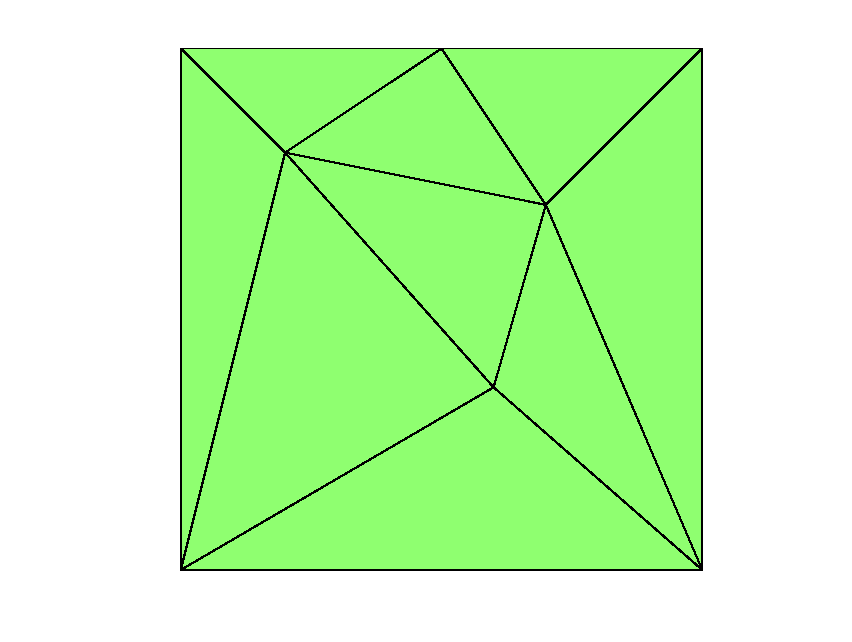
\includegraphics[width=0.15\textwidth]{6DL/figures/unstructureGrid.pdf} &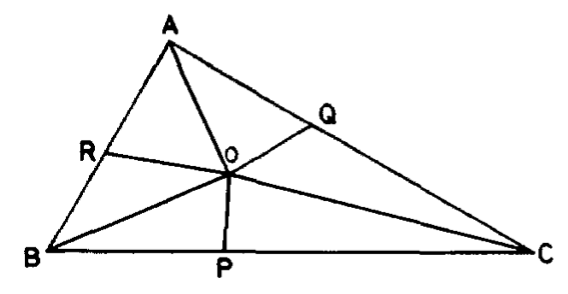
\includegraphics[width=0.22\textwidth]{6DL/figures/PowellSabin2.png} &$\cdots$ & \\
Conjecture: $k=(m-1)2^d+1$  &  Powell-Sabin \cite{powell1977piecewise}&  $\cdots$ & ReLU$^m$-DNN \\
True: $d=1,m\ge 1$ &    $k=2$ &   $\cdots$ & $k=m$     \\
$d=2,m=2$ (Still open)  & $d=2,m=2$ & $?$&  any $d$ and $m$ \\
\hline
\end{tabular}
\caption{Competitions between locality and global smoothness.}
\label{compare}
\end{table}
\end{center}
Observation: More global d.o.f. lead to easier
construction of conforming elements for high order PDEs.

\subsection{Piecewise $P_m$ for $H^m(\Omega)$: from finite element to
  finite neuron method} \label{sec:concluding} As it is noted above,
in the classic finite element setting, it is challenging to construct
$H^m$-conforming finite element spaces for any $m, d\ge 1$.  But if we
relax the conformity, as shown in \cite{wang2013minimal}, it is
possible to give a universal construction of convergent
$H^m$-nonconforming finite element consisting of piecewise polynomial
of degree $m$.  In the finite neuron method setting, by relaxing the
constraints from the a priori given finite element grid, the
construction of $H^m$-conforming piecewise polynomials of degree $m$
becomes straightforward.  In fact, the finite neuron method can be
considered as mesh-less method, or even, vertex-less method although
there is a hidden grid for any finite neuron function.  This raises a
question if it is possible to develop some "in-between" method that have
the advantages of both the classic finite element method and the
finite neuron method. 

\subsection{Adaptivity and spectral accuracy} 
One of the important properties in the traditional finite element
method is its ability to locally adapt the finite element grids to
provide accurate approximation of PDE solution that may have local
singularities (such as corner singularities and interface
singularities).  In contrast, the traditional spectral method (using
high order polynomials) can provide very high order accuracy for
solutions that are globally smooth.  The finite neuron method analyzed
in this paper seems to possess both the adaptivity feature as in the
traditional finite element method and also the global spectral
accuracy as in the traditional spectral methods.  Adaptivity feature
of the finite neuron method is expected since, as shown in 
\S~\ref{sec:deep-fnm},  the deep finite neuron method can recover locally
adaptive finite element spaces for $m=1$.  Spectral feature of the
finite neuron method is illustrated in Theorem~\ref{thm:spectral}.
As a result, tt is conceivable that the finite neuron method may have both the
local and also global adaptive feature, or perhaps even adaptive
features in all different scales.  Nevertheless, such highly adaptive
features of the finite neuron method come with a potentially big
price, namely the solution of a nonlinear and non-convex optimization
problems.

\subsection{Comparison with PINN}
One important class of methods that is related to the FNM analyzed in
this paper is the the method of physical-informed neural networks
(PINN) introduced in \cite{raissi2019physics}.  By minimizing
certain norms of PDE residual together with penalizations of boundary
conditions and other relevant quantities, PINN is a very general
approach that can be directly applied to a wide range of problems.  In
comparison, FNM can only be applied to some special class of problems
that admit some special physical laws such as principle of energy
minimization or principle of least action, see \cite{feynmanfeynman}.
%\footnote{ Chapter 19
%  of Volume II, Feynman R, Leighton R, and Sands M. The Feynman
%  Lectures on Physics . 3 volumes 1964, 1966. Library of Congress
%  Catalog Card No. 63-20717. ISBN 0-201-02115-3 (1970 paperback
%  three-volume set); ISBN 0-201-50064-7 (1989 commemorative hardcover
%  three-volume set); ISBN 0-8053-9045-6 (2006 the definitive edition
%  (2nd printing); hardcover)}.  
Because of the special physical law associated with our underlying
minimization problems, the Neumann boundary conditions are naturally
enforced in the minimization problem and, unlike in the PINN method,
no penalization is needed to enforce such type of boundary conditions.

\subsection{On the sharpness of the error estimates} 

We  note our error estimate \eqref{error:D} for Dirichlet boundary
condition is not as good as the one \eqref{error:N} for Neumann
boundary conditions.  This is undesirable and may not be optimal.  In
comparison, Nitsche trick does not suffer a loss of accuracy when used
in traditional finite element method.

\subsection{Neural splines in multi-dimensions}
The spline functions described in Section~\ref{sec:Bsplines} are widely
used in scientific and enginnering computing, but their generalization
multiple dimension are non-trivial, especially when $\Omega$ has
curved boundary. In \cite{hu2015minimal}, using the tensor product,
the authors extended the 1D spline to multi-dimensions on rectangular
grids.  Some others involve rational functions such as NURBS
\cite{cottrell2009isogeometric}. But the generalization of neural networks to multi-dimension is straightforward and also the
resulting (nonlinear) space has very good approximate properties.  It
is conceivable that the neural network extension of B-spline to
multiple dimensions which are locally polynomials and globally smooth,
may find useful applications in computer aid design (CAD) and
isogeometric analysis \cite{cottrell2009isogeometric}. This is a
potentially an interesting research direction.




